\documentclass[tikz,convert={outfile=\jobname.svg}]{standalone}

\usepackage[utf8]{inputenc}
\usepackage{amsmath}
\usepackage{minted}
\usepackage{tipa}
\usepackage{tikz}

\begin{document}
\def\sx{43} \def\sy{-55} \def\ex{55} \def\ey{-35}
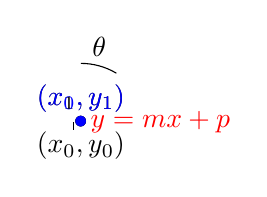
\begin{tikzpicture}[scale=0.125]
    \draw (\sx, \sy) node{$\bullet$} node[below]{$(x_0, y_0)$};
    \draw (\ex, \ey) node{$\bullet$} node[above]{$(x_1, y_1)$};
    \draw[blue] (\sx, \sy) -- (\sx, \ey) node{$\bullet$} node[above]{$(x_0, y_1)$};
    \draw[red] (\sx, \sy) -- (\ex, \ey) node[right,midway]{$y = mx+p$};
    \draw (\sx+0.25, \ey) -- (\sx+0.25, \ey+0.25);
    \draw (\sx+0.25, \ey+0.25) -- (\sx+0.25, \ey);
    \draw (\sx, \sy+7) arc (90:59:7) node[above,midway]{$\theta$};
\end{tikzpicture}

\end{document}
